\chapter{On Multimedia Analysis and Retrieval}
\epiquote{All our knowledge begins with the senses, proceeds to the understanding, and ends with reason.}{Immanuel Kant}
\label{chapter:theory_multimedia_analysis_and_retrieval}

Multimedia data is ubiquitous and used in different forms in every area of our daily lives, be it private or professional. Statista.com estimates, that the amount of data created, captured, copied, and consumed in 2025 will exceed \SI{181000}{\exa\byte} from an estimated \SI{2000}{\exa\byte} in 2010\footnote{Source: Statista.com, ``Volume of data/information created, captured, copied, and consumed worldwide from 2010 to 2025'', February 2022}. To a large extent, that data is multimedia data, which is being uploaded and shared on social media and the Internet.

A key development in this regard was the broad adoption of the smartphone in the early 2000s, which enabled almost every person on this planet to not only consume but also produce multimedia content in the form of texts, images, videos and audio snippets and to share those on platforms such as Twitter, Instagram, Facebook or TicToc turning them effectively into prosumers \cite{Ritzer:2010Production,Ritzer2012:Coming}. Fueled by this technological progress, the past few decades have seen a staggering development in both \emph{volume} and \emph{variety} of multimedia data found in the wild and in private data collections.

This extreme growth as well as the increasing \emph{velocity} at which data is being produced, poses an enormous challenge for information processing, analysis and retrieval systems that deal with multimedia. Therefore, researchers have tried to tackle the questions surrounding the efficient and effective management, analysis and retrieval of multimedia data at large scales for many decades now, with first attempts reching back to the early 70s.

\section{Multimedia Data and Multimedia Collections}
\label{section:multmedia_data}

The term \emph{multimedia} refers to a combination of one or many different \emph{media types}, such as but not limited to, aural or visual information. We distinguish between these types, based on the representation we use when working and interacting with them. Sound, for example, is formed by airpressure waves that are registered by our ears. In contrast, visual information, involves electormagnetic waves captured by our eyes. In both cases, the brain plays an important role in interpreting the underlying processes and forming the human perception of the phenomenon. Similarily, we rely on different techniques when converting these media types from their analogue to their digital representations. 

Traditionally, we often think of media as information that somehow can be perceived directly by our human senses. However, we consider (multi-)media data in a wider sense, which may also include less apparent and sometimes even digitally native examples such as motion capture data or data streams stemming from sensors or medical devices. 

Even though the various media types may exhibit very different characteristics in their original representation, we find some commonalities that are crucial for formalising the problem of processing and analysing such data in information processing systems in general and analytics and retrieval systems in particular (see Examples \ref{example:representation_visual_information} and \ref{example:representation_audio_information}).

\begin{description}
    \item[Relationship with Time] At a high level, we can roughly classify all the different media types based on their relationship with time. \emph{Static} media types (e.g., an image) do not exhibit a temporal development, whereas the information in \emph{dynamic} media types (e.g., an audio signal) depends on the time point that is being examined \cite{Blanken:2007multimedia}.

    \item[Unstructured Data] The digital representation of any media type is typically highly unstructured, thus, there is no natural data model that can be leveraged for analysis. For example, there is generally no apparent connection between the raw image data and the motives it depicts. Therefore, information processing systems rely on \emph{derivative representations} of the original data, gained through pre-processing and data analysis.
    
    \item[Semantic Gap] The derivative representations of the original data usually describe specific aspects thereof and conversion to/from such representations is therefore often accompanied by a loss of information. This is a problem often referred to as the \emph{semantic gap} \cite{Blanken:2007multimedia, Rossetto:2018thesis}.
\end{description}

\begin{example}[label=example:representation_visual_information]{Digital Representation of Visual Information}{}
    \begin{wrapfigure}{L}{0.45\textwidth}
        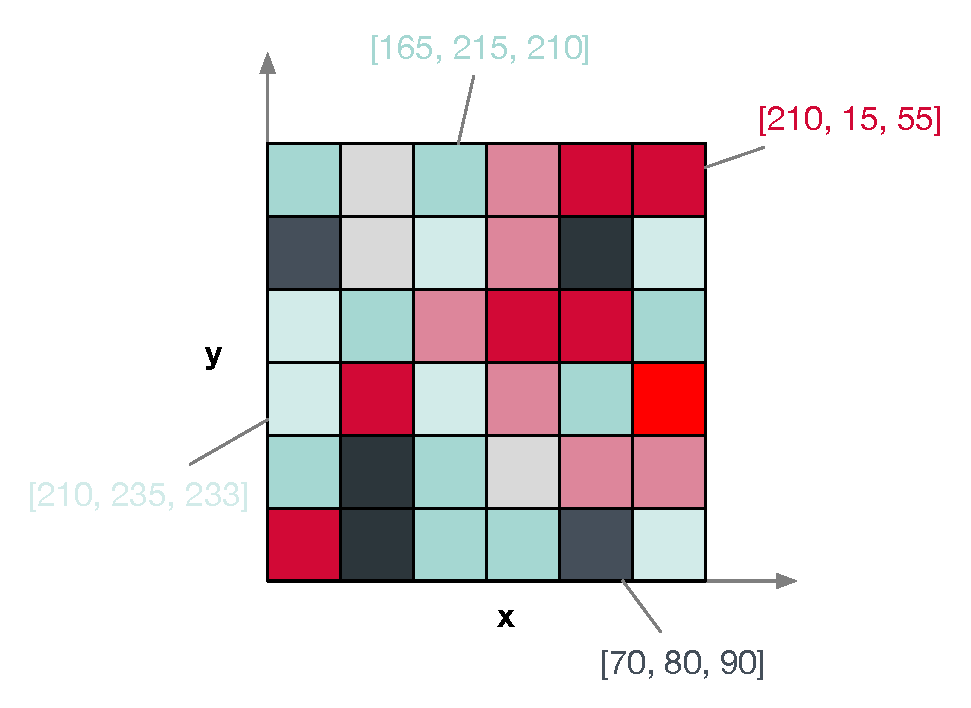
\includegraphics[width=0.45\textwidth]{figures/example-visual-signal.eps}
    \end{wrapfigure}
    The visual information in a flat image is stored as a two dimensional array of \emph{pixels}. The information in every pixel is typically formed by a sensor, in an array of sensors, that captures the electormagnetic signal. Each pixel holds colour values, usually one per colour channel. For example, with the RGB colour model, every pixel holds three values, one for the red, green and blue channel. The number of pixels per dimension determines the \emph{resolution} of the image. Typically, we use a fixed number of bits per colour -- the \emph{colour depth} -- which determines the number colours that can be distinguished.

    If we take, for example, a coloured image of $1000 \times 1000$ pixel, we must encode \num{3e6} individual colour values. Using \SI{8}{\bit} per colour, we end up storing \SI{24e6}{\bit}, which amounts to \SI{3}{\mega\byte} worth of uncompressed image data. Images coming from modern cameras, exhibit resolutions much higher than that.
\end{example}

\begin{example}[label=example:representation_audio_information]{Digital Representation of Aural Information}{}
    \begin{wrapfigure}{R}{0.45\textwidth}
        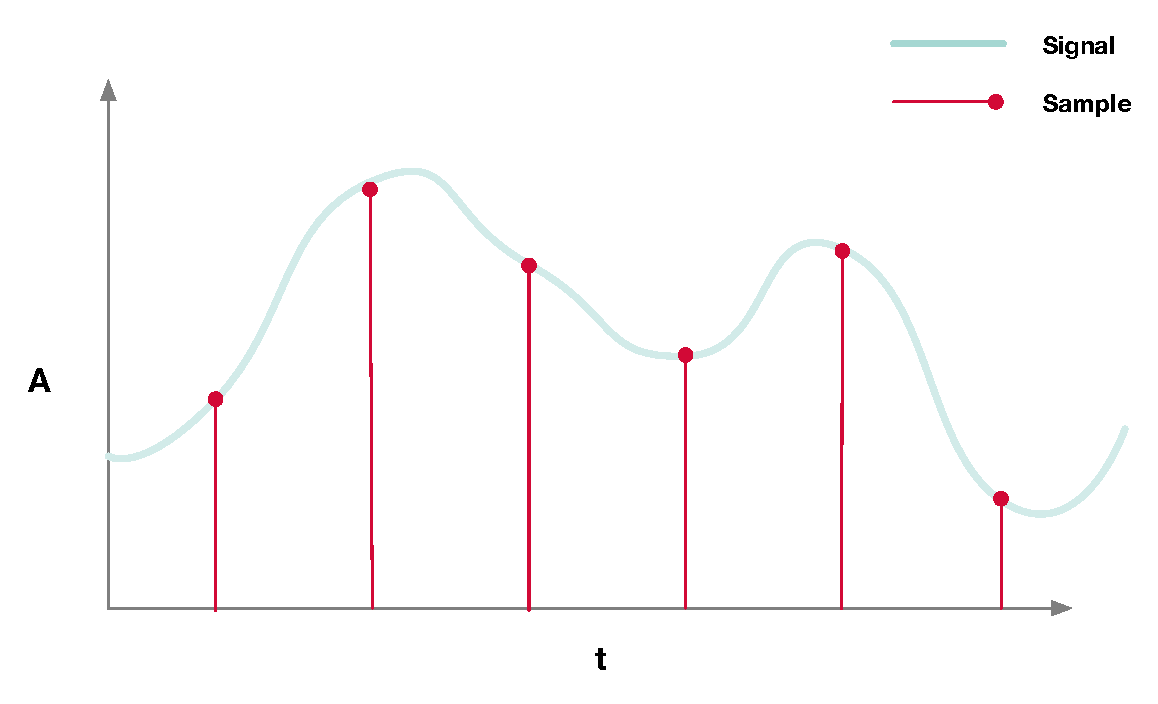
\includegraphics[width=0.45\textwidth]{figures/example-audio-signal.eps}
    \end{wrapfigure}
    The airpressure waves that form sound can be recorded and translated to an electrical signal by microphones. When digitizing this information, the temporal development of this signal amplitude is \emph{sampled} at a fixed rate. Each sample point consist of a value that quantizes the amplitude's energy at a given point in time to a number on a given range. An audio stream is then a sequence of these values. The quality of the process is determined by the \emph{sample rate}, i.e., the number of samples per time unit, and the \emph{bit depth}, which determines quantization of the amplitude power.

    If we take a \SI{1}{\second} audio snippet, sampled at \SI{44}{\kilo\hertz}, we end up storing \num{44000} sample points. Using a bit depth of \SI{16}{bit} per sample, this amounts to \SI{704000}{\bit} or \SI{88}{\kilo\byte} of uncompressed audio data. In modern audio systems, we typically record multiple audio channels independently, leading to even more data.
\end{example}

\subsection{A Data Model for (Multi-)Media Data}
\label{section:media_data_model}
In \Cref{chapter:theory_databases}, we have introduced the notion of a data model and its importance for working with any type of data. Despite being agnostic to the concrete, conceptual data model in principle, the work presented in this Thesis still relies on a formal understanding of media data that enables organisation and management thereof. Due to its tight integration into the \emph{vitrivr} project \cite{Rossetto:2016vitrivr,Gasser:2019Multimodal,Heller:2020Multi}, there is a particular model that we would like to introduce. Under this data model -- which is illustrated in \Cref{figure:erm_mediadata_vitrivr} -- a (multi-)media collection consists of multiple \emph{media object}s. The media object describes the data at the level of individual documents -- e.g., a video or image file -- and comprises of basic attributes such its identifier, its media type or its path. The path forms the link to the raw media data in the filesystem, which we assume to be the most suited form of storage for this type of information. 

To account for the temporal development found in dynamic media types, \emph{vitrivr}'s data model has a notion of a \emph{media segment}, which represents a clearly defined, temporal slice of the object and stands in a one-to-many relationship with it. However, the model does not make any assumption as to how segments are formed. For static media types, such as images, there is a trivial one-to-one relationship between an object and a segment. For more complex media types, such as audio or video, \emph{media segmentation} is a dedicated area of research \cite{Koprinska:2001temporal} and can be approached in many different ways, e.g., at a fixed rate, based on changes in the content \cite{Foote:2000Automatic,Tsai:2016video} or using self-adaptive, deep neural networks~\cite{Souvcek:2019transnet}. Obiviously, different strategies for segmentation yield different degrees of summarization of information over time. Additionally, the proposed distinction also allows for very application specific media types and segmentation strategies, such as \emph{image sequences} -- introduced for \acrshort{lsc} 2020 \cite{Heller:2020Interactive} -- which group related images per day for the purpose of lifelog analysis.

To model the different derivative representations that are used to describe a media object and its segments, the model foresees \emph{features}, which again stand in a one-to-many relationship with the segments. That is, every segment can have an arbitrary number of such features that describe different aspects of the segment's content. In practice, different types of features are obtained and stored in dedicated entities. Additionally, \emph{descriptive metadata} allows for a description of the media both at the document and segment level by means of simple key-value pairs containing descriptions or labels.

\begin{figure}[bt]
    \centering
    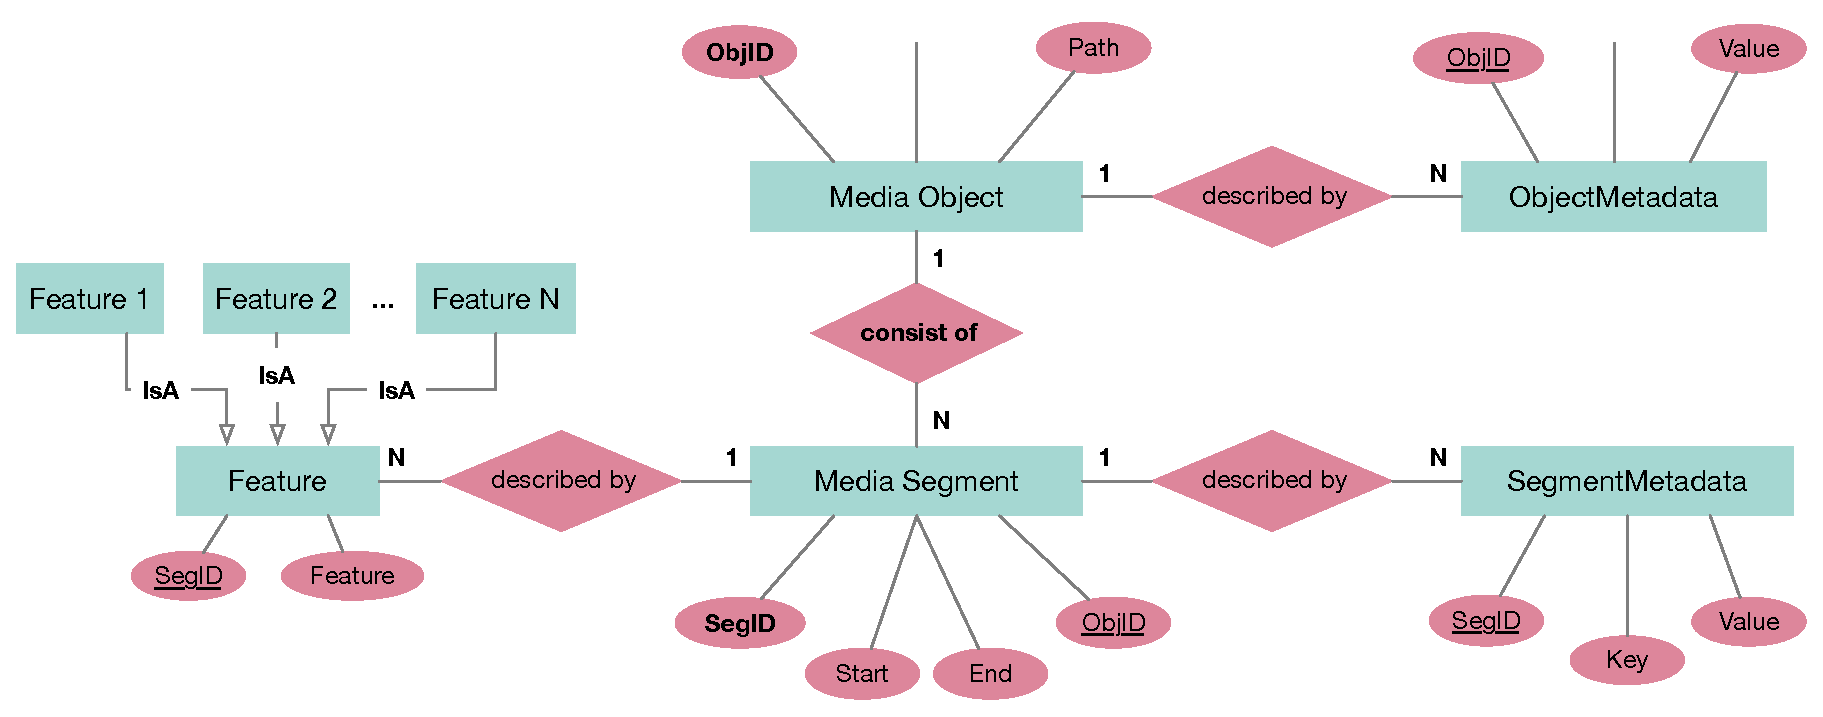
\includegraphics[width=\textwidth]{figures/erm-media-data-vitrivr}
    \caption{An extended \acrshort{erm} of the multimedia data model used in the \emph{vitrivr} project. The model is centered around the notion of media objects and media segments which are described by metadata and features.}
    \label{figure:erm_mediadata_vitrivr}
\end{figure}

While proven to be useful, the proposed model is only one possible approach to model media data and media collections and in  certain aspects. 

For the purpose of this Thesis, we consider a slightly altered version of the aforementioned data model, which is more in line with \cite{Blanken:2007multimedia} and is illustrated in \Cref{figure:erm_mediadata}. This model also considers media objects to be an abbstraction of individual files. However, this model foregoes the indirection introduced by the media segment and treats \emph{features}, \emph{annotations} and \emph{descriptions} as different types of a more general \emph{metadata} type that describes the media object directly. To model the temporal aspect in dynamic media types, the metadata itself exhibits information about the part of the object that is being described, denoted by an optional \emph{start} and an \emph{end} marker. In practice, this could be a frame number or a timestamp.

While the difference between the two models may seem marginal, we argue, that the latter offers several advantages over the former: Firstly, it eliminates a level of indirection introduced by the media segment and thus simplifies handling of static media types, which are simply described by different types of metadata that lack a start and end marker. Secondly, it does not assume segmentation to be statically defined and instead makes this a property of the metadata itself. This is reasonable, because the optimal segmentation strategy may depend on a particular feature, especially when multiple media types are involved, e.g., aural and visual information in a video. And finally, the model could be extended to also support spatial information as basis for segmentation, e.g., in images, which would enable description of spatio-temporal aspects of any media type. However, such ideas are beyond the scope of this Thesis. 

We will use the proposed, conceptual data model from \Cref{figure:erm_mediadata} throughout this Thesis and whenever we refer to terms like collection, media object, feature or descriptive metadata, we refer to the concepts introduced in this model.

\begin{figure}[bt]
    \centering
    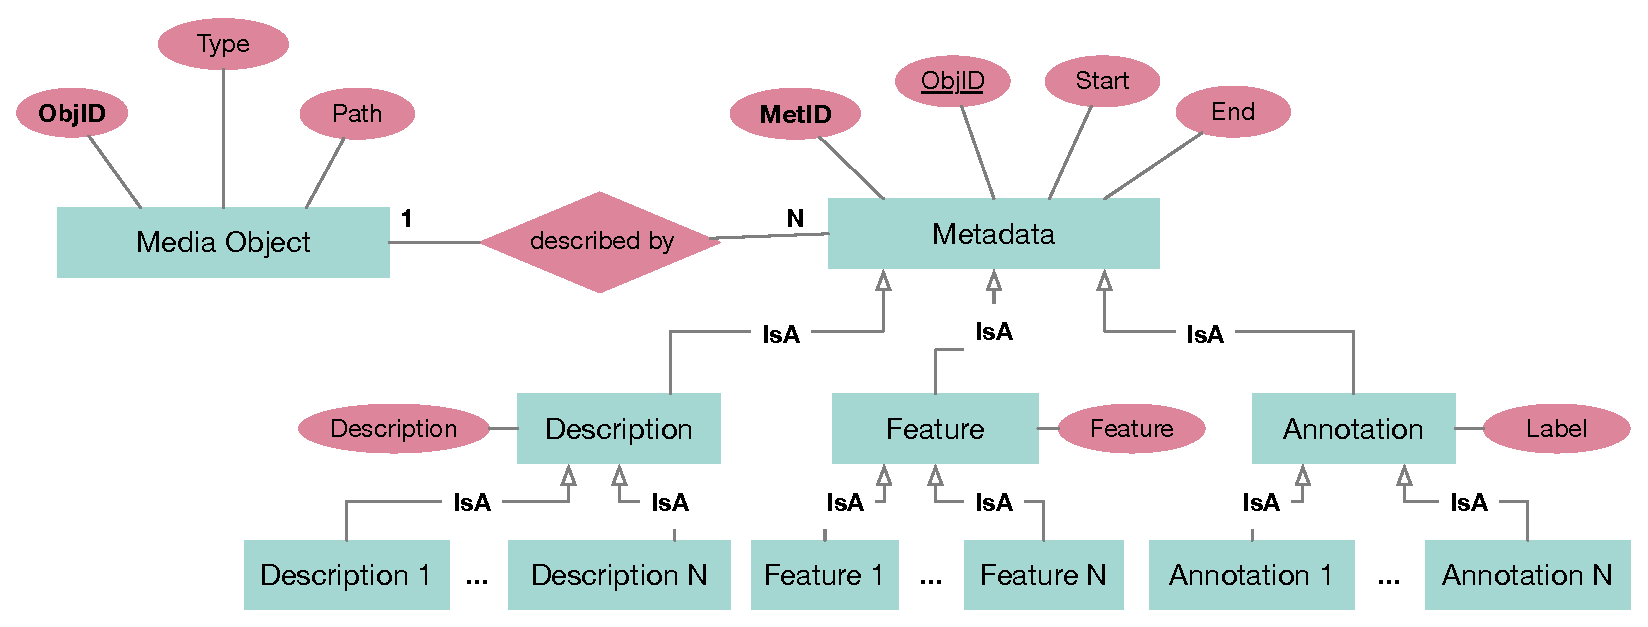
\includegraphics[width=\textwidth]{figures/erm-media-data}
    \caption{An extended \acrshort{erm} of the multimedia data model used for the purpose of this Thesis. It has been derived from \emph{vitrivr}'s data model and foregoes the explicit segment entity.}
    \label{figure:erm_mediadata}
\end{figure}

\subsection{Descriptive Metadata}
Descriptive metadata in the sense of the proposed data model comprises of textual descriptions (e.g, title, summary), technical information (e.g., duration, location, frame rate) and annotations (e.g., category labels). Such information has always played an important role in multimedia retrieval and analysis, because it provides (indirect) access to the media's content and can be leveraged in a structured way, e.g., in database queries or for data organisation.

Over the years, many different metadata standards have emerged. For example, ID3\footnote{See https://id3.org/} tags allow for organisation of large music libraries and classification of songs based on information about artists or albums. Similarily, the Dublin Core Metadata Element Set (DCMES or just Dublin Core)\footnote{See https://www.dublincore.org/} comprises of 15 basic properties that can be used to describe any type of media, e.g., videos or images. And last but not least, EXIF\footnote{See https://www.loc.gov/preservation/digital/formats/fdd/fdd000146.shtml/} can be used to describe images and also includes technical metadata, such as the camera model, the exposure time or the f-number. These well established standards are complemented by a plethora of domain specific, standardised and non-standardised metadata frameworks.

However, while useful and important for the problem of analysis and retrieval, this type of metadata comes with important disadvantages. Firstly, and notwithstanding recent developments in machine learning, e.g., in image captioning \cite{Hossain:2019Comprehensive}, such information is traditionally assigned manually in a laborious and time-consuming annotation process. This process is barely able to keep up with the ever increasing velocity at which new content is created. Secondly, descriptions and labels -- especially if not standardised -- are often subjective due to language, expertise and personal experience and may therefore differ depending on the person assigning them. This is closely related to the problem of the perceptive- and interpretative gap \cite{Rossetto:2018thesis} and highly relevant for any search process. And finally, it is often challenging to describe the content of media in a textual manner, especially if temporal development is involved.\todo{We use this often. But is there some study on this?}

Regardless of these challenges, however, experience shows that annotations -- be they assigned manually or automatically -- play an important role, especially when it comes to information retrieval. A contributing factor here is that of query formulation, which is very low-effort and familiar for textual input and becomes more challenging for other types of queries \todo{Source}.

\subsection{Features}
Simply put, a \emph{feature} is a mathematical object that describes ``derived characteristics''~\cite{Blanken:2007multimedia} of a media object or a part thereof. Therefore, they are sometimes also referred to as \emph{descriptors}. A formal definition is given in \Cref{definition:feature}.

\begin{definition}[label=definition:feature]{Definition of a Feature in Multimedia Analysis}{}
    Let $\symmediacol = \lbrace o_1, o_2, \ldots, o_N \rbrace$ be a media collection of media objects $o$ (i.e., files). A \emph{feature} $f_{i,\texttt{start},\texttt{end}} \in \symfeatures$ describes a temporal interval $[ \texttt{start}, \texttt{end} ]$ with $\texttt{start},\texttt{end} \in \symnatural_0, \texttt{start} \leq \texttt{end}$ of the media object $o_i \in \mathcal{C}$ under the feature transformation $\symfeaturetransform$, with 

    \begin{equation}
        \label{eq:feature_transformation}
        \symfeaturetransform \colon \mathcal{C} \times \symnatural_0 \times \symnatural_0 \longrightarrow \mathcal{F}
    \end{equation}

    We call $\symmediacol$ the media object domain and $\symfeatures$ the feature domain. The structure of  $\symfeatures$ is fully determined by $\symfeaturetransform$.
\end{definition}

Features play a central role in many different domains, ranging from mere (multi-)media analysis to retrieval. \cite{Blanken:2007multimedia} distinguishes between low-level and high-level features, which is a qualitative assesment of how far removed the derived characteristic of a particular feature is from a concept that has a semantic meaning to a human user. For example, a histogram of the colours found in an image would be considered a low-level feature, whereas a feature capturing salient keypoints or even objects in the same image would be classified as high-level. In practice, high-level features are often derived from low-level features, and again these conversions are subject to the semantic gap.

The process of generating features from media objects is called \emph{feature extraction} \cite{Blanken:2007multimedia} and there is an entire corpus of research that deals with the engineering of features that describe the relevant aspects of a given media type's content, with first attempts in computer vision and image understanding dating back to the early 60s. Various surveys, such as \cite{McKinney:2003Features,Ding:2012ASurvey,Salau:2019Feature}, cover the topic of feature extraction and we simply name and describe a few selected examples to provide an (unrepresentative) overview. Obviously, every type of media has their own analysis technqiues that can be used to generate features.

For images, one can roughly distinguish between low-level colour, texture and shape features \cite{Salau:2019Feature}, as well as higher-level local keypoint-based features. An example of a colour feature could be a simple colour histogram or a statistical moment that captures colour distribution, e.g., the average colour in a defined area of the image. Prominent examples for keypoint detection features include algorithms such as \acrfull{sift}~\cite{Lowe:1999object}, \acrfull{surf}~\cite{Bay:2006surf} or \acrfull{hog}~\cite{Dalal:2005Histograms}. All these features are employed in many different applications ranging from retrieval and similarity search to the detection of higher-level concepts, such as, objects or faces \cite{Deniz:2011Face, Farooq:2016Object}.

Similarily, there is a wide range of features applied in audio analysis and retrieval. \acrfull{mfcc} -- a representation of a short-term power spectrum on the perceptual \emph{mel scale} -- play an important role in speaker recognition, sound and music classification as well as audio segmentation \cite{Kim:2010Comparison} and were shown to outperform audio descriptors outlined in the MPEG-7 standard~\cite{Quackenbush:2001Overview}, which is a collection of standardised feature descriptors for images, audio and video. Other types of features include \acrfull{pcp} for music retrieval and classification~\cite{Lee:2006Automatic,Demirel:2019Automatic} or features based on rhythm, timbre or speed. 

So far, we have mostly considered features that were engineered through the careful application of signal processing and/or statistical analysis of the raw media data. However, advances in machine learning and deep neural neutwork architectures have enabled the feature extraction process to be automated to some extend, leading to a shift from  engineered to learned features \cite{Hamel:2010Learning,Gordo:2016Deep}. There is also research that deals with the comparison of the two paradigms in multimedia retrieval and analysis \cite{Budnik:2017learned} as well as other domains, such as chemical structure analysis \cite{Gallegos:2021importance}. Preliminary results show, that while learned features often outperform the engineered ones, best results are attained by a combination of the two.

Given the cornucopia of features and feature extraction techniques to chose from, there are two important aspects that ought to be considered with respect to data modeling and data management: First, and despite the vast range of feature extraction techniques, the resulting features often exhibit a comparatively simple mathematical structure. We will show in \Cref{section:multimedia_retrieval} that in multimeda retrieval, one often deals with vectors in a high-dimensional, real-valued vector space \cite{Zezula:2006Similarity}. Second, when considering a complex enough use-case, no single feature can satisfy all the different types of applications because, as we as have pointed out, a specific feature usually focuses on a specific aspect of the content. Consequently, a combination of features often yields the best results \cite{Deselaers:2008Features}.

Both these aspect have important implications for the the requirements on a data management and processing system for multimedia data, especially, if such a system should be able support different use-cases that are not necessarily known in advance. We would also like to point out, that both data models introduced in \Cref{section:media_data_model} are flexible enough to handle these two aspects.

\section{Multimedia Retrieval}
\label{section:multimedia_retrieval}

\emph{Multimedia retrieval} deals with algorithms, methods and systems that allow for content-based search and obtaining items of interest from large (multi-)media collections based on user-defined queries. In addition to text-based search, such queries may also involve new modes of query formulation such as \emph{Query-by-Example} \cite{Kelly:1995Query}, \emph{Query-by-Sketch} \cite{Cao:2010mind}, \emph{Query-by-Humming} \cite{Ghias:1995query} or \emph{Query-by-Sculpting} \cite{Boerlin:20203d}. Many different research domains for the different types of media have emerged over the years, including but not limited to image retrieval \cite{Dharani:2013Survey}, audio retrieval \cite{Lu:2001Indexing}, video retrieval \cite{Hu:2011Survey}, 3D model retrieval \cite{Yang:2007Content} and various, specialised subdomains \cite{Murthy:2018Content}.

Formally, the multimedia retrieval problem can be charactersied finding all media objects $o \in \symmediacol$ that may be relevant to a given \emph{information need} expressed by a user as query $Q$. This is achieved by obtaining some form of \emph{(dis-)similarity}\footnote{Depending on the context, the similarity of an object to a query may be directly or inversely proportional to the obtained score, which is what makes the difference.} between $Q$ and $o$ and ranking results based on it, which is why the method is also referred to as \emph{similarity search}. In contrast to Boolean search, the results of similarity search are non-binary in the sense that an object $o$ may match a query $Q$ only to a certain degree but still be considered part of the resultset, as opposed to a strict match / no-match semantic.

Since a direct comparison of a media object to a query is often not feasible -- for reasons described in \Cref{section:multmedia_data} -- features are used as a proxy instead. This is a manifestation of the idea that derivative representations are considered in lieu of the actual object, leading to the formal \Cref{definition:similarity_search} of similarity search.

\begin{definition}[label=definition:similarity_search]{Definition of the General Similarity Search Problem}{}
    Let $\symmediacol = \lbrace o_1, o_2, \ldots, o_N \rbrace$ be a media collection of media objects $o$ and let further $\symfeatures$ be a feature domain of $\symmediacol$ under the feature transformation $\symfeaturetransform$. Furthermore, we assume a query $Q$ that can be mapped to $\symfeatures$, i.e., $\symfeaturetransform(Q) = q \in \symfeatures$ and the existence of an inverse $\symfeaturetransform^{'}$ with $\symfeaturetransform^{'}(f) = o$ \footnote{While this may seem like a wild assumption at first, this is a given since we explicitly store the relationship between $o$ and $f$, according to the data model in \Cref{section:multmedia_data}.}.

    Similarity search then is the optimisation problem of finding the object $o \in \symmediacol$ that given a query $q$ and a similarity function $\symsim \colon \symfeatures \times \symfeatures \rightarrow [0, 1]$ maximises the following expression.

    \begin{equation}
       o_r =  \symfeaturetransform^{'} (\argmax_{f \in \symfeatures} \symsim(f,q))
    \end{equation}
 
    We call the resulting item $o_r$ most similar w.r.t. to $Q$, which is indicated by the similarity score $\symsim(f,q)$. In practice, we may be interested in the top $k$ results rather than just a single item.
\end{definition}

In simple terms, a multimedia retrieval system operates upon features $f \in \symfeatures$ derived from the original media objects by means of a feature transformation. This transformation is applied twice: Once when indexing a media object in the collection -- often a step that is thought as taking place offline -- and once when deriving the same feature from the query input $Q$ provided by the user. Subsequently, the system generates the similarity measure $\symsim(q,f)$ which quantifies the similarity between $q$ and $f$ from low ($0.0$) to almost identical ($1.0$). The flow of information that results from this approach is illustrated in \Cref{figure:multimedia_retrieval_flow}. 

In many cases, the function $\symsim$ may not express similarity but dissimilarity between objects, in which case we can simply consider the dual problem. Furthermore, the score may not always be normalized to $[0, 1]$, which makes it difficult to combine scores of multiple features, e.g., in \emph{score-based late fusion} \cite{Depeursinge:2010Fusion,Rossetto:2018thesis}. However, a normalised similarity score can always be derived by applying an additional correspondence function $\symcorr \colon \symreal \rightarrow [0, 1]$. Both aspects are of high practical relevance but do not change the fundamental problem definition. 

\begin{figure}[tb]
    \centering
    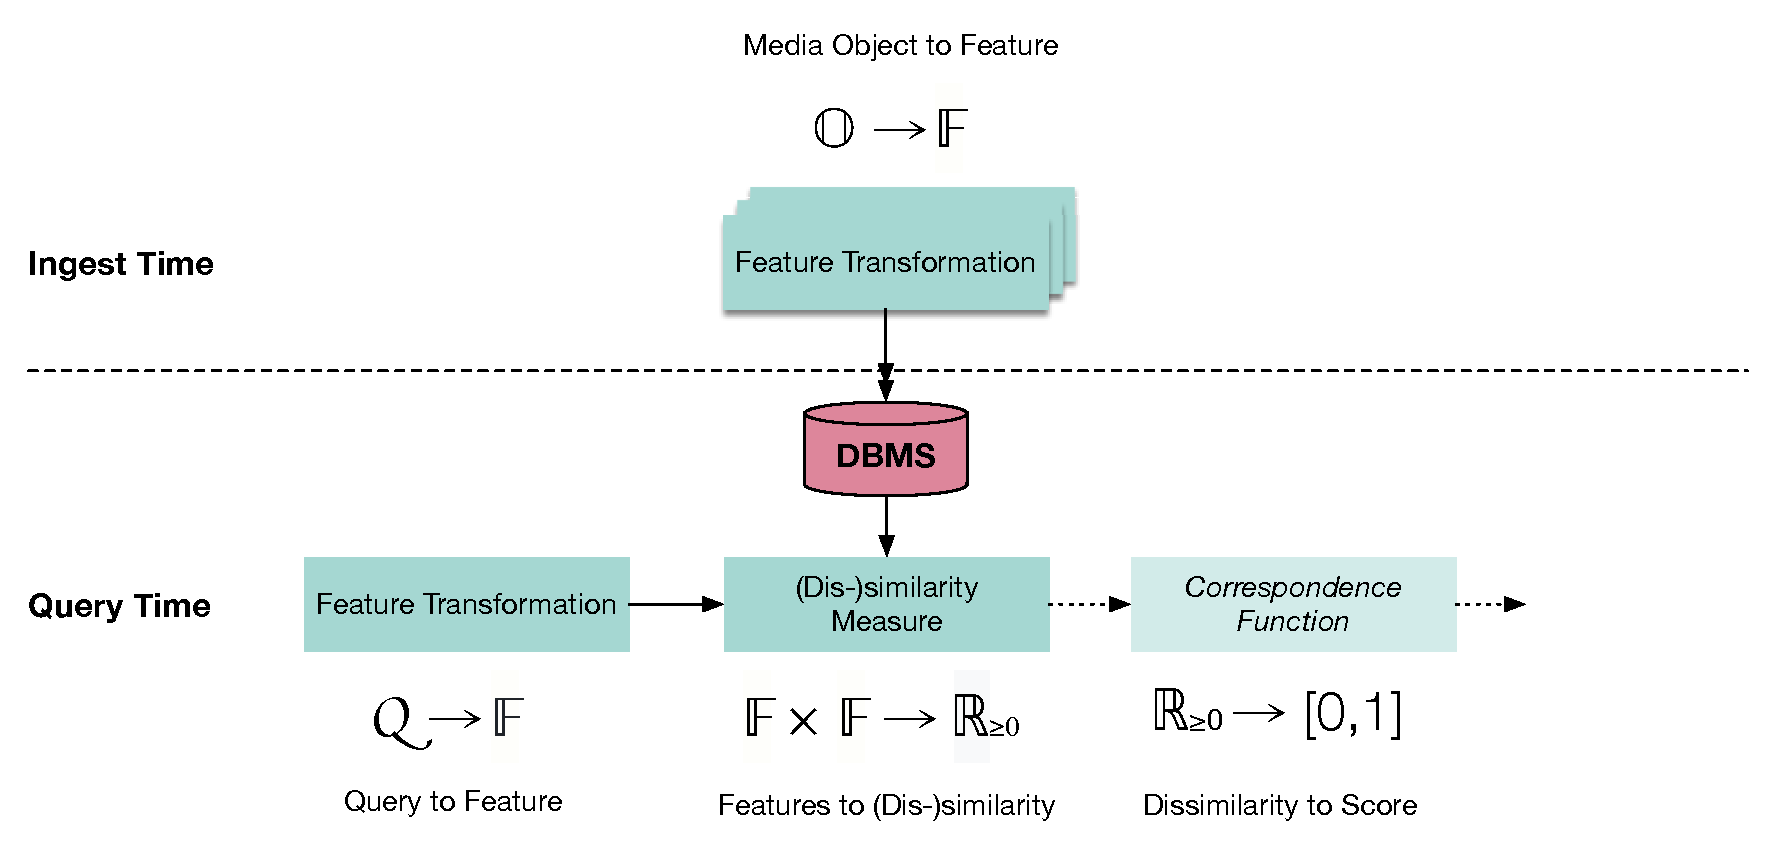
\includegraphics[width=\textwidth]{figures/multimedia-retrieval-pipeline}
    \caption{Flow of information in similarity search at ingest- and query time.}
    \label{figure:multimedia_retrieval_flow}
\end{figure}

\subsection{Similarity Search and the Vector Space Model}

The \emph{vector space model} of similarity search assumes that the domain of the feature vectors $\symfeatures$ is a subset of a mathematical vector space -- that is, a set whose elements may be added and multiplied by a scalar. In practice, we often consider that vector space to be real-valued and high-dimensional, i.e., $\symfeatures \subset \symreal^{d}$ wherein $d$ is the dimension and an inherent property of the feature and the underlying transformation $\symfeaturetransform$. Consequently, every feature $f \in \symreal^{d}$ is simply a point in that high-dimensional vector space.

Under this premise, we consider the dissimilarity function $\symdist(f,q)$ to be a function that calculates the distance between a feature and a query $f,q \in \symfeatures$, as defined by \Cref{eq:distance_function}. Typically, the farther two vectors lie apart under the distance measure, the more dissimilar they are, which is why we also call this proximity based search. A list of important distance functions used in similarity search is given in \Cref{table:similarity_measures}. 

\begin{equation}
    \label{eq:distance_function}
    \symdist \colon \symfeatures \times \symfeatures \rightarrow \symreal
\end{equation}

\begin{table}[hb]
    \begin{tabular}{ | c | c | c | c | c | c |}
        \hline
        \textbf{Name} & \textbf{Symbol} &  $\symdist \mathbf{(f,q)}$ & \textbf{Domain} & \textbf{Co-Domain} & \textbf{Metric} \\
        \hline
        \hline 
        Manhattan & $L^1$ & $\sum_{i=1}^{d} | f_i - q_i |$ & $\symreal^d$ & $\symreal$ & metric \\ 
        \hline
        Euclidean & $L^2$ & $\sqrt{\sum_{i=1}^{d} (f_i - q_i)^2}$ & $\symreal^d$ & $\symreal$ & metric \\  
        \hline
        Minkowski & $L^p$ & $\sqrt[p]{\sum_{i=1}^{d} (f_i - q_i)^p}$ & $\symreal^d$ & $\symreal$ & metric if $p \in \symnatural_{\geq 1}$ \\ 
        \hline
        Chi-Square & $\chi^2$ & $\sum_{i=1}^{d} \frac{(f_i - q_i)^2}{f_i + q_i}$ & $\symreal^d$ & $\symreal$ & metric \\ 
        \hline
        Kullback-Leibler & - & $\sum_{i=1}^{d} q_i \log (\frac{q_i}{f_i})$ & $\symreal^d$ & $\symreal$ & non-metric \\ 
        \hline
        Cosine & - & $1 - \frac{\sum_{i=1}^{d} f_{i}q_{i}}{\sqrt{\sum_{i=1}^{d} f_i^2} \sqrt{\sum_{i=1}^{d} q_i^2}}$ & $\symreal^d$ & $[-1, 1]$ & semi-metric \\  
        \hline
        Jacccard & - & $1 - \frac{A \cap B}{A \cup B}$ & $\symfeatures$ & $[0, 1]$ & metric \\
        \hline
        Levenshtein & - & - & $\mathbb{S}$ & $\symnatural$ & metric \\
        \hline
        Hamming & - & - &  $\mathbb{S}$ & $\symnatural$ & quasi-metric \\
        \hline
        LCS \cite{Hirschberg:1977Algorithms} & - & - &  $\mathbb{S}$ & $\symnatural$ & non-metric \\
        \hline
    \end{tabular}
    \caption{List of distance functions often used in similarity search.}
    \label{table:similarity_measures}
\end{table}

At a high level, one can distinguish between \emph{continuous} and \emph{discrete} distance functions \cite{Zezula:2006Similarity}. Continuous functions typically exhibit a very large, potentially infinite co-domain wheras discrete functions map to a limited, often pre-defined set of values. For example, the \emph{Euclidean distance} is a continuous distance function, whereas the \emph{Levenshtein distance} \cite{Levensthtein:1965Binary} is discrete.

Furthermore, we can distinguish between metric distance functions that induce a topology on the underlying vector space -- often denoted as $(\symfeatures, \symdist)$ -- as opposed to functions that do not. A metric distance function satisfies the \emph{non-negativity}, \emph{symmetry}, \emph{identity of indiscernables} and \emph{triangle inequality} constraints and $(\symfeatures, \symdist)$ is called a \emph{metric space}. 

\begin{align}
  \label{eq:metric}
   \symdist(f,q) &\geq 0                           \tag{non-negativity} \\
   \symdist(f,q) &= \symdist(q,f)                    \tag{symmetry}\\
   \symdist(f,q) &= 0 \Longleftrightarrow f = q    \tag{identity of indiscernables}\\
   \symdist(f,q) &\leq  \symdist(f,g) +  \symdist(g,q)   \tag{triange inequality}\\
   \forall f,g,q \in \symfeatures \wedge (\symfeatures, \symdist) \nonumber
\end{align}

The constraints imposed on a metric space give rise to mathematical properties that can be exploited for efficient execution of similarity search and specialised indexing techniques \cite{Zezula:2006Similarity}. However, despite their mathematical convenience, some applications involve distances that do not exhibit all the aforementioned properties of a metric, e.g., quasi-metrics (lack symmetry), semi-metrics (lack triangle inequality), meta-metrics (lack identity) \cite{Zezula:2006Similarity} or even necessitate the use of non-metric functions \cite{Skopal:2011Nonmetric}.

The choice of (dis-)similarity measure mainly depends on the application. All the Minkowski distances, (i.e., $L^1$, $L^2$, $L^p$) can be used for any type of real-valued vector and in practice, it often makes little difference which one is employed \cite{Rossetto:2018thesis}. Of all the Minkowski distances, the Euclidean distance ($L^2$) is the most common. The Chi-squared distance is well suited, if the feature vectors represent histgrams \cite{Pele:2010Quadratic}. The Hamming- and Levenshtein distances belong to the class of \emph{edit distances} and can be used to compare strings.

Regardless of what (dis-)similarity measure is selected, the similarity search problem always looks as defined in \Cref{definition:similarity_search}: Given a query $q \in \symfeatures$, the search algorithm should return all features $o \in \symmediacol$ whose features $f = \symfeaturetransform(o)$ lie within a given proximity or distance to the query object $q$ and that further satisfy the selection condition. Depending on this selection condition, we distinguish between different types of similarity search problems \cite{Zezula:2006Similarity}. Those are illustrated in \Cref{fig:sim_search_algorithm} and \Cref{example:similarity_search}

\subsubsection{\acrfull{nns}}

\acrshort{nns} is probably one of the most prominent types of queries used in multimedia retrieval and certainly the one employed most often in the context of the \emph{vitrivr} \cite{Rossetto:2016vitrivr,Gasser:2019Multimodal} stack. Given the query object $q$ and an arbitrary limit $k \in \symnatural$ the task is to find the $k$ features $f \in \symfeatures$ that are closest to $q$ as illustrated in \Cref{fig:knn}. This is also referred to as \acrfull{knn}. Formally, the resultset $R$ is given by \Cref{eq:knn}.

\begin{equation}
    \label{eq:knn}
    \lbrace R \subset \symfeatures \colon \forall f_r \in R, f \in \symfeatures \setminus R, \symdist(q,f_r) \leq \symdist(q,f) \wedge |R| = k \rbrace
\end{equation}

Algorithmically, the distance between all $f \in \symfeatures$ and $q$ must be evaluated exhaustively and the top $k$ results must be retained by ranking and ordering the results, e.g., in a \emph{bound priority queue}. This is sometimes referred to as \emph{brute-force} approach to \acrshort{nns}. For $\symfeatures \subset \symreal^d$, its runtime complexity is $\mathcal{O}(dN)$ and thus depends linearly on the cardinaltiy $N = |\symfeatures|$ and the dimension $d$. 

A variant of \acrshort{knn} is \acrfull{kfn} wherein instead of the nearest, the farthest neighbours are obtained. This can be useful, for example, to obtain negative examples to train recommender systems \cite{Pagh:2015Approximate}. However, the underlying algorithm remains the same.

\subsubsection{Range Search}

The range query or $\epsilon$NN is useful for finding objects that lie within a given range, typically expressed by a value $\epsilon \in \symreal$. Given the query object $q$, the task is to find all features $f \in \symfeatures$ that lie within $\epsilon$ of $q$ as illustrated in \Cref{fig:enn}. Formally, the resultset $R$ is given by \Cref{eq:epsilonnn}.

\begin{equation}
    \label{eq:epsilonnn}
    \lbrace R \subset \symfeatures \colon \forall f_r \in R, \symdist(q,f_r) \leq \epsilon \rbrace
\end{equation}

Algorithmically, this search strategy is similar to \acrshort{nns} in that all features must be evaluated exhaustively and in that its complexity for $\symfeatures \subset \symreal^d$is $\mathcal{O}(dN)$. However, in contrast to \acrshort{nns}, there is no need for intermediate sorting, since the selection is based on a simple, numerical comparison to the constant $\epsilon$.

Variants of $\epsilon$NN include instances, where $f$ must be larger than $\epsilon$ or where $f$ must fall into an interval $[ \epsilon_{lower}, \epsilon_{upper} ]$. However, these variants are equivalent to the base-case since only the selection predicate changes.

\subsubsection{\acrfull{rnns}}

In \acrshort{rnns} we try to find all $f \in \symfeatures$ that given a limit $k \in \symnatural$ consider the query $q \in \symfeatures$ to be part of their \acrshort{knn} resultset as illustrated in \Cref{fig:rknn}. Formally, the resultset $R$ is given by \Cref{eq:rknn} 

\begin{equation}
    \label{eq:rknn}
    \lbrace R \subset \symfeatures \colon \forall f_r \in R, q \in \texttt{kNN}(f_r) \wedge f \in \symfeatures \setminus R \colon q \in \texttt{kNN}(f)  \rbrace
\end{equation}

Algorithmically, this type of search is more complex than \acrshort{knn} or $\epsilon$NN, because basically, a \acrshort{nns} problem must be solved for every element $f \in \symfeatures$. Therefore, the runtime complexity is $\mathcal{O}(dN^2)$ and scales with the square of $N = |\symfeatures|$. 

\begin{example}[label=example:similarity_search]{Comparing different types of similarity search algorithms}{}
    For this example, we consider $\symfeatures \subset \symreal^2$ and $f \in \symfeatures$ to be points of interest (e.g., museums, hotels, parks) on a two-dimensonal city map. Furthermore, we consider $q \in \symfeatures$ to be another position on the same map, e.g., given by our current position or a selected point of interest. The different types of similarity queries can now be thought of as follows:

    \begin{description}
        \item[Nearest Neighbour Search] is the equivalent of finding the $k$ points of interest that are closest to $q$ (e.g., the three museums closest to my location).
        \item[Range Search] is the equivalent of finding all points of interest that are within $\epsilon$ distance from  $q$ (e.g., all museums within \SI{3}{km} from my location).
        \item[Reverse Nearest Neighbour Search] is the equivalent of finding all points of interest that consider $q$ to be among their closest points of interest (e.g., finding all hotels that have a specific museum in the set of their three closest sites that must be seen when visiting the city).
    \end{description}
\end{example}

\begin{figure}
    \centering
    \begin{subfigure}[b]{0.25\textwidth}
        \centering
        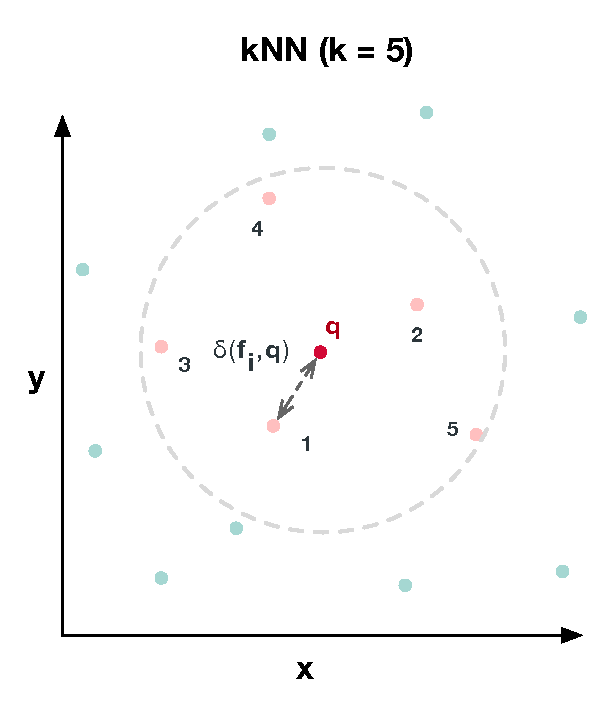
\includegraphics[width=\textwidth]{figures/knn}
        \caption{kNN}
        \label{fig:knn}
    \end{subfigure}
    \hfill
    \begin{subfigure}[b]{0.25\textwidth}
        \centering
        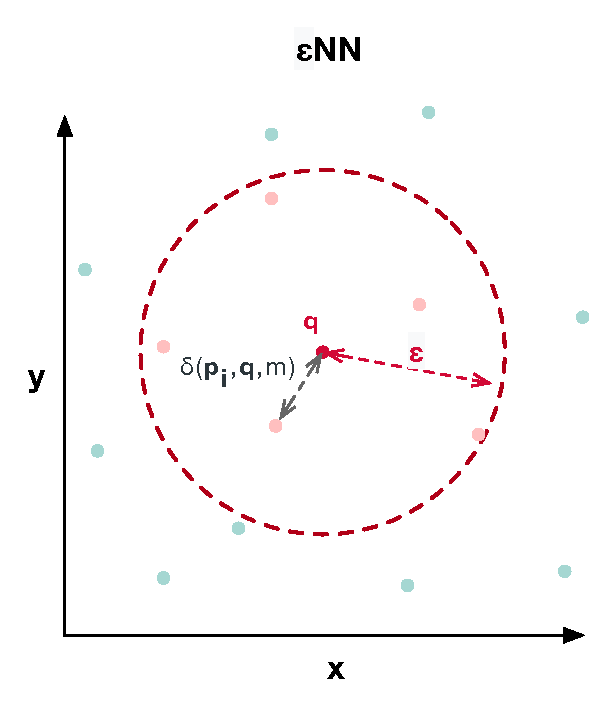
\includegraphics[width=\textwidth]{figures/enn}
        \caption{$\epsilon$NN}
        \label{fig:enn}
    \end{subfigure}
    \hfill
    \begin{subfigure}[b]{0.25\textwidth}
        \centering
        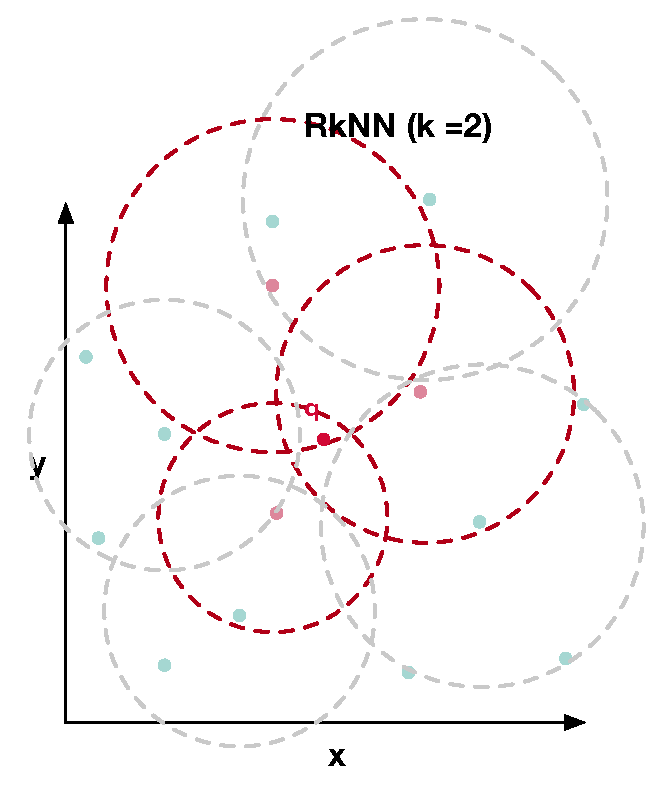
\includegraphics[width=\textwidth]{figures/rknn}
        \caption{RkNN}
        \label{fig:rknn}
    \end{subfigure}
    \caption{Illustration of the different similarity search algorithms in $\symfeatures \subset \symreal^2$ using the Euclidean distance ($L^2$). Matches are highlighted in red.}
    \label{fig:sim_search_algorithm}
\end{figure}

\subsection{\acrshort{nns} and High-Dimensional Index Structures}

As we have argued in \Cref{section:multimedia_retrieval}, even the simple \acrshort{nns} problem in $\symreal^d$ exhibits a non-negligible runtime complexity of $\mathcal{O}(dN)$ for a linear, brute-force scan -- thus being proportional to the cardinality of $N = |\symfeatures|$ and the dimension $d$. Experience from database research shows that linear scans are too slow in terms of time required for query execution if $N$ becomes large enough, especially when interactive query workloads are involved. This necessitates the use of index structures that allow for sub-linear data access.

For search in high-dimensional vector spaces, the dependency on $d$ has a huge impact on execution performance of any \acrshort{nns} algorithm, due to what is known as the \emph{curse of dimensionality} \cite{Indyk1998:Approximate,Zezula:2006Similarity}. The impact of this ``curse'' is twofold: First, the execution time of a brute-force algorithm is directly proportional to the size of the feature vector. With a tendency towards more complex and thus higher-dimensional vectors, there is a direct, negative effect on runtime. Second, and more importantly, research has shown that the task of indexing high-dimensional vectors for more efficient access is not trivial and that traditional approaches, e.g., based on partitioning or classical tree structures, degenerate as dimensionality increases \cite{Indyk1998:Approximate,Weber:1998Va} with the consequence, that they only yield marginal or no improvement over executing a linear scan. In fact, it was formally proven by \cite{Shaft:2006Theory} in their \emph{Theory of Nearest Neighbor Indexability} that the performance of almost all known index structures at that time deteriorate to that of a linear scan if $d$ becomes large enough.

Nevertheless, the issue of index structures that allow for more efficient and thus sub-linear \acrshort{nns} has been taken on by various researchers over the past few decades with results of high practical relevance. At a high-level, indexing algorithms can be classified along three dimensions: First, based on whether they provide any guarantees w.r.t. to the accuracy of the results, wherein ``accuracy'' is often measured in terms of precission and recall of a result produced by an index as compared to the the result produced by a linear scan \cite{Echihabi:2021High}. Second, based on their \emph{structure} \cite{Shaft:2006Theory}, e.g., \emph{list}, \emph{tree}, \emph{graph}, \emph{hash table} and \emph{inverted file}. And finally, by the method that is employed, e.g., \emph{quantization}, \emph{hashing} or \emph{partitioning}. An overview of different, prominent algorithms is provided in \Cref{table:index_structures}.

\begin{table}
    \begin{tabular}{ | l | c | c | c |}
        \hline
        \textbf{Name} & \textbf{Guarantees} & \textbf{Structure} & \textbf{Method} \\
        \hline
        \hline
        KDB-Tree \cite{Robinson:1981KDB} & exact & tree & space partitioning \\  
        \hline
        $R^{*}$-Tree \cite{Beckmann:1990RTree} & exact & tree & data partitioning \\ 
        \hline
        \acrshort{vaf} \cite{Weber:1998Va} & exact & list & quantization \\ 
        \hline
        VA+ \cite{Ferhatosmanoglu:2000Vector} & exact & list & quantization \\ 
        \hline
        \acrshort{lsh} \cite{Indyk1998:Approximate, Wang:2017ASurvey} & approximate, probabilistic & hash table i.a.  & hashing \\ 
        \hline
        \acrshort{pq} \cite{Jegou:2010Product} & approximate & inverted file & quantization \\ 
        \hline
        NV-tree \cite{Lejsek:2009NVTree} & approximate & tree & quantization \\ 
        \hline
        MRNG \cite{Lejsek:2009NVTree} & approximate & graph & proximity graph \\ 
        \hline
        HSNW \cite{Malkov:2018Efficient} & approximate & graph & proximity graph \\ 
        \hline
    \end{tabular}
    \caption{Non-representative and non-exhaustive list of high-dimensional index structures employed in similarity search and retrieval.}
    \label{table:index_structures}
\end{table}

Early examples of high-dimensional indexes used to rely on space or data partitioning methods. Both have in common, that they assign features in the vector space to buckets or data files based on some partitioning of either the vector space or the data. Space partitioning methods include but the KD-Trees \cite{Bentley:1975Multidimensional}, KDB-Trees \cite{Robinson:1981KDB} or Quadtrees \cite{Finkel:1974Quad}. The data partitioning methods involve R-Trees \cite{Guttmann:1984RTrees}, $R^{*}$-Trees \cite{Beckmann:1990RTree} or M-Trees \cite{Ciaccia:1997Mtree}. All of these methods were shown to perform well as long as dimensionality remains small (i.e., 4 to 12 dimensions) but they tend to deteriorate as $d$ increases.

In the next few sections, we will highlight a few more recent examples of high-dimensional indexing methods to provide a non-representative overview.

\subsubsection{\acrfull{vaf}}

VA-files were first proposed by Weber et al. \cite{Weber:1998Va} to address the problem of the dimensionality curse and were later refined by \cite{Ferhatosmanoglu:2000Vector}. The basic idea of a \acrshort{vaf} is the division of the data space into $2^b$ cells, as illustrated in \Cref{fig:vaf}, where $b$ denotes a fixed number of bits. Typically, one choses a specific number of bits per dimension $b_d$ and uniformly partitions the vector space along each dimension, i.e., $b = b_dd$. A feature vector's position in the grid is concatenated into a compact \emph{signature} of size $b$ and the VA-file is a list of those signatures. 

\begin{figure}[bt]
\centering
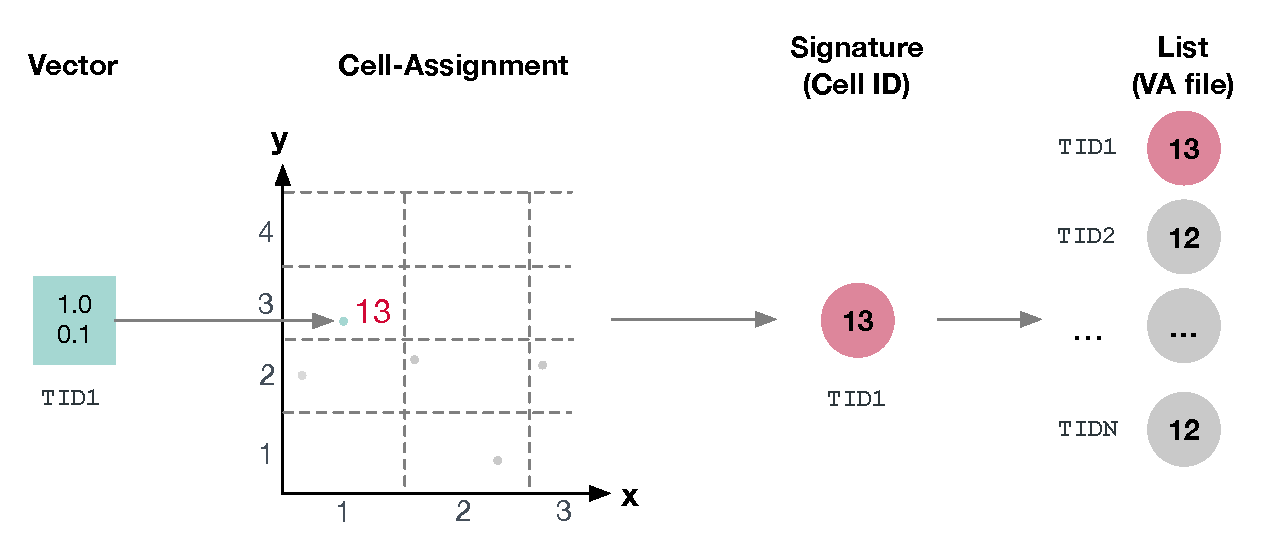
\includegraphics[width=0.95\textwidth]{figures/vaf}
\caption{Simplified illustration of basic \acrshort{vaf} indexing scheme in for $\symfeatures \subset \symreal^2$. A vector is assigned to a cell which gives rise to a signature that is stored in a linear list.}
\label{fig:vaf}
\end{figure}

\acrshort{nns} is then realised as a linear scan of the file. Speed-up over a linear scan of the original vectors is achieved in two ways: Firstly, the signatures are more compact than the original representation, which reduces IO cost through compression. Secondly, the signatures can be used to obtain approximate bounds that are computationally less expensive than the actual distance calculation. These bounds can be used to filter out a majority of the points in the file, further reducing IO and CPU costs. Experimental results presented in \cite{Weber:1998Va} demonstrate that 90\% of all features can be skipped thus a distance must only be obtained for the remaining 10\%. However, \cite{Echihabi:2021High} determine theoretically that for \acrshort{vaf} degeneration is to be expected nevertheless for high dimensions, depending on how the data is distributed.

The VA+-files proposed by \cite{Ferhatosmanoglu:2000Vector} introduce a few optimisations to the original algorithm. They suggest a prior decorellation of the individual dimensions by applying a \emph{Karhunen-Loève Transform} and a dynamic assignment of bit per dimension based on data distribution as opposed to a uniform distribution proposed in the original paper.

\subsubsection{\acrfull{lsh}}

\acrshort{lsh} refers to a family of algorithms \cite{Echihabi:2021High,Wang:2017ASurvey} that all share the same, basic idea of \emph{locality preserving hashing} as first proposed by \cite{Indyk1998:Approximate}. The idea is centered around a hash function $h: \symfeatures \rightarrow B$ that maps any two points $f,q \in \symfeatures$ to a bucket $b \in B$ such that Equations \ref{eq:lsh_1} and \ref{eq:lsh_2} hold, wherein $(\symfeatures, \symdist)$ must constitute a metric space, $P_1, P_2 \in [0, 1], P_1 > P_2$ denote probabilities, $R > 0$ denotes an arbitrary threshold and $c > 1$ denotes an approximation factor.

\begin{eqnarray}
    \symdist (p,q) \leq R \Rightarrow h(f) = h(q) \text{ with a probability of at least } P_1 \label{eq:lsh_1} \\
    \symdist (p,q) \geq cR \Rightarrow h(f) = h(q) \text{ with a probability of at most } P_2 \label{eq:lsh_2}
\end{eqnarray}

In simple terms, a locality preserving hash function has a high probability for collision (i.e., mapping to the same bucket) if two features $f,q \in \symfeatures$ lie close to one another, i.e., $\symdist(q,f) \leq R$, but exhibits a low probability for collision if $\symdist(q,f) \geq cR$. Given such a hash function, a feature $f \in \symfeatures$ can be hashed to a bucket and stored in a hash table with other vectors that lie close to it. This is illustrated in \Cref{fig:lsh}. 

Speedup for \acrshort{nns} can be achieved by limiting distance calculation to the vectors in the bucket a query $q$ falls into. This is referred to as non-exhaustive search. However, due to the probabilistc nature of the hash function, this type of search strategy may exhibit errors due to vectors that were hashed into the ``wrong'' bucket. More refined strategies can be employed including hash-code ranking as well as single- and multi-table lookup \cite{Wang:2017ASurvey} to further minimize that error. Nevertheless, \acrshort{lsh} remains an approximate search strategy. A survey of different LSH algorithms can be found in \cite{Wang:2017ASurvey}.

\begin{figure}[bt]
    \centering
    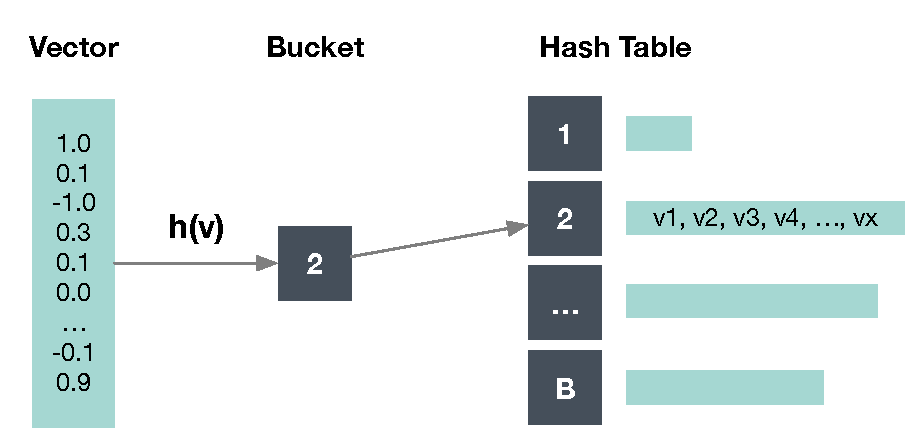
\includegraphics[width=0.95\textwidth]{figures/lsh}
    \caption{A simplified illustration of the basic \acrshort{lsh} indexing scheme. A vector is hashed to a bucket by a locality preserving hash function $h$. The vector is then stored in the assigned bucket in a hash table.}
    \label{fig:lsh}
\end{figure}

\subsubsection{\acrfull{pq}}

The idea for \acrshort{pq} was proposed by \cite{Jegou:2010Product} and it describes a technique for quantizing vectors. The main idea involves decomposition of the original vector space $\symreal^d$ into smaller subspaces $\symreal^s$ with $s < d$ and separate quantization of each subspace. The quantization is achieved by learning a codebook for every subspace through k-means clustering on a representative sample of the data. Upon indexing, all subvectors of each feature vector $f \in \symfeatures$ are assigned to the nearest centroid in the codebook for the respective subspace. Concatenation of the centroid indexes gives rise to a compact signature that can be stored in an inverted file index, as illustrated in \Cref{fig:pq}.

\begin{figure}[bt]
    \centering
    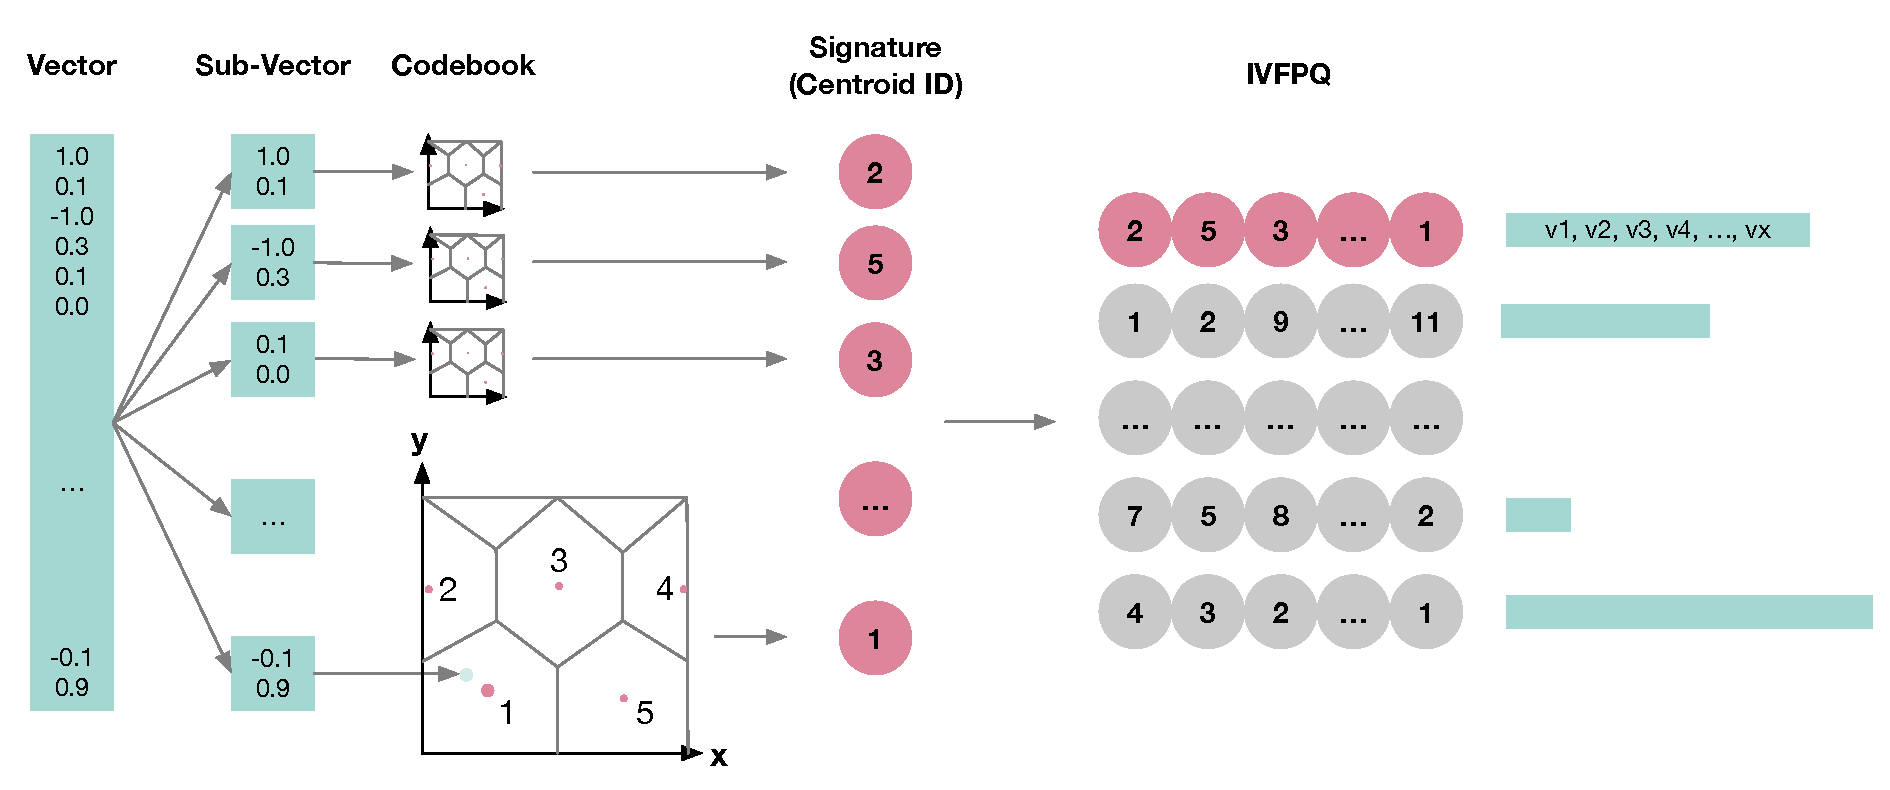
\includegraphics[width=0.95\textwidth]{figures/pq}
    \caption{A simplified illustration of the basic \acrshort{pq} indexing scheme. A vector is divided into smaller subvectors and each subvector is assigned to the nearest centroid in the codebook of the respective subspace. Concatenating the resulting centroid index per subspace gives rise to the signature, which can be stored in an inverted file index.}
    \label{fig:pq}
\end{figure}

Speedup of \acrshort{nns} is achieved in two ways: First, the resulting signature is a highly compressed representation of the original vector, which reduces IO by a large margin as is demonstrated in \Cref{example:pq_compression}. Secondly, the signature can be used directly to approximate the distance between a query $q$ and a feature $f$ using a pre-calculated lookup-table and inexpensive operations, which reduces CPU costs. However, this speedup must be bought by a distortion of the approximated distance, which may lead to errors if features lie very close to one another and makes PQ a suboptimal fit if exact distance values are required.

\cite{Jegou:2010Product} also discusses several optimisations that can be employed, e.g., encoding the residuals instead of the actual feature vectors to increase accuracy or to use multiple levels of coarse quantizers to introduce an additional partitioning of the data in very large data collections.

\begin{example}[label=example:pq_compression]{Size of PQ-Signature vs. original feature}{}
    Let us assume $\symfeatures \subset \symreal^{256}$, i.e., a $256$-dimensional vector space ($d = 256$). Assuming a \texttt{float} data type, we require \SI{4}{\byte} per vector component, i.e., \SI{1024}{\byte} to store a single vector.
    
    Using \acrshort{pq}, this space could now be divided into $16$ subspaces with a dimensionality of $16$ each, i.e., $s = 16 < d$. If now we assume, that we create a codebook consisting of $128$ clusters for each subspace, then every subvector will be assigned to one of $128$ centroids, which will result in $16$ numbers (one per subspace) between $0$ and $127$. Each of these numbers can be stored in a single \texttt{byte}, that is, we only need \SI{16}{\byte} per vector to store an index entry.
\end{example}

\subsection{Beyond Similarity Search}
In real-world multimedia retrieval systems, the query workloads are far more diverse than what we have described so far. In addition to ``simple'', one-shot queries, users find themselves searching, refining, browsing and exploring datasets with the aim to find a particular item \cite{Lokovc:2019Interactive,Rossetto:2020Interactive}. This is exemplified by interactive retrieval competitions such as \acrfull{vbs} \cite{Schoeffmann:2019Video,Lokovc:2018Influential} or \acrfull{lsc} \cite{Gurrin:2021Introduction}, where participants are required to find items of interest in large, standardised data collections \cite{Berns:2019V3C1,Rossetto:2021Insights} within a limited amount of time.

The various participants have demonstrated interesting techniques that complement and replace mere similarity search. While the 2022 iteration was won by a system combining search using the CLIP model \cite{Radford:2021Learning} and sophisticated browsing \cite{Hezel:2022Efficient}, the team behind \cite{Kratochvil:2020SOM} has won the 2020 iteration of \acrshort{vbs} with a system that relies on \acrfull{som} \cite{Kohonen:1990Self} to generate a clustered visualisation of the high-dimensonal data collection initialised by search input. Similarily, the system that won in 2016 used \cite{Barthel:2016Navigating} hierarchical graphs and visually sorted image maps to facilitate exploration without providing any classical search functionality. Generally, it was found that efficient browsing is as important for effective retrieval as an effective similarity search model \cite{Lokovc:2019Interactive}. Another comparison of systems at the \acrshort{lsc} 2018 has shown, that a combination of functionality that complements similarity search is very common, including functions such as Boolean search on biometric data, facet filters and visual clustering. \cite{Gurrin:2019Invited}. Hence, as argued in \Cref{section:application_retrieval}, multimedia retrieval goes way beyond mere similarity search but always relies on it to some extent.